% Figure macros for Chapter 4 (Results).

\newcommand{\figResultsOverview}{%
\begin{figure}[!htbp]
\centering
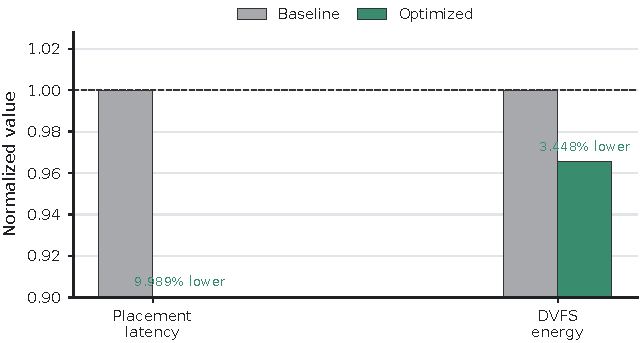
\includegraphics[width=0.86\linewidth]{figures/results_overview.pdf}
\caption{Overview of the two main evaluation outcomes. Placement reports normalized latency relative to HEFT, while DVFS reports normalized energy relative to no-DVFS execution. The y-axis is truncated to make the normalized differences visible.}
\label{fig:results-overview}
\end{figure}%
}

\newcommand{\figBenchmarkCopyVolume}{%
\begin{figure}[!htbp]
\centering
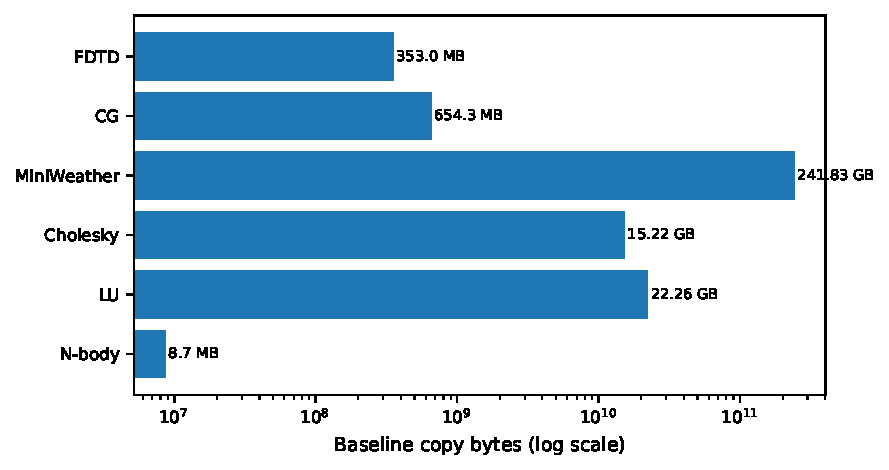
\includegraphics[width=0.86\linewidth]{figures/benchmark_copy_volume.pdf}
\caption{Baseline copy volume for the benchmark suite. The log-scale x-axis separates absolute copy traffic from residual-placement opportunity: MiniWeather has large baseline copy volume, but the placement measurements show little reducible copy traffic under the residual policy.}
\label{fig:results-benchmark-copy-volume}
\end{figure}%
}

\newcommand{\figPlacementDeltas}{%
\begin{figure}[!htbp]
\centering
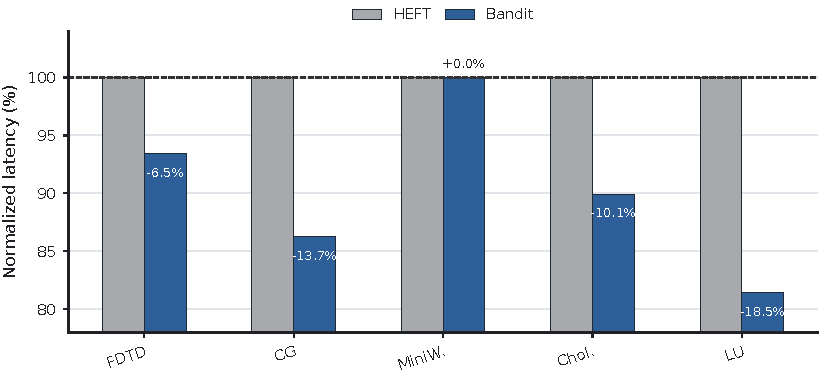
\includegraphics[width=0.94\linewidth]{figures/placement_deltas.pdf}
\caption{Normalized placement latency relative to HEFT. HEFT is fixed at \(100\%\) for each benchmark, and the Bandit bars show the corresponding normalized latency reduction.}
\label{fig:results-placement-deltas}
\end{figure}%
}

\newcommand{\figCopyLatencyScatter}{%
\begin{figure}[!htbp]
\centering
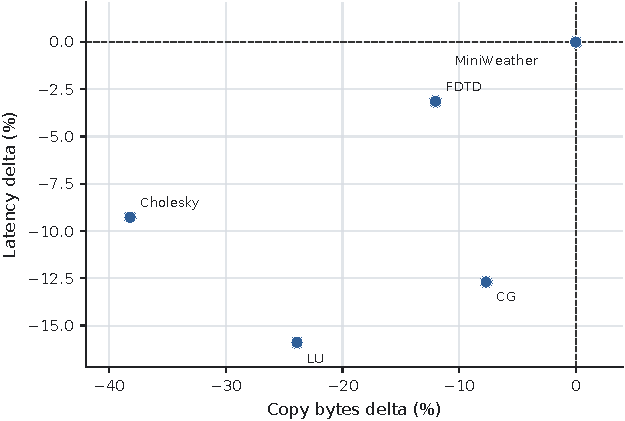
\includegraphics[width=0.78\linewidth]{figures/copy_latency_scatter.pdf}
\caption{Relationship between copy-byte reduction and placement latency reduction. CG uses copy counters from the placement measurements because the locality diagnostic set does not include a CG deviation-rate row.}
\label{fig:results-copy-latency}
\end{figure}%
}

\newcommand{\figDeviationLatencyScatter}{%
\begin{figure}[!htbp]
\centering
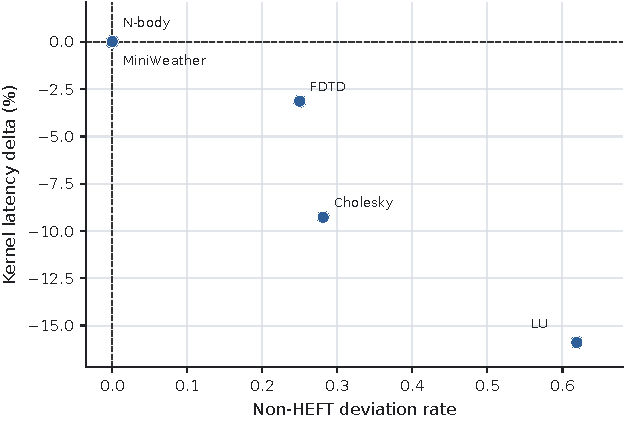
\includegraphics[width=0.78\linewidth]{figures/deviation_latency_scatter.pdf}
\caption{Scheduler deviation rate and placement latency improvement in the locality diagnostic measurements. Deviation frequency is explanatory, not a direct linear predictor of speedup. CG is omitted because the diagnostic set does not contain its deviation-rate row.}
\label{fig:results-deviation-latency}
\end{figure}%
}

\newcommand{\figDvfsDeltas}{%
\begin{figure}[!htbp]
\centering
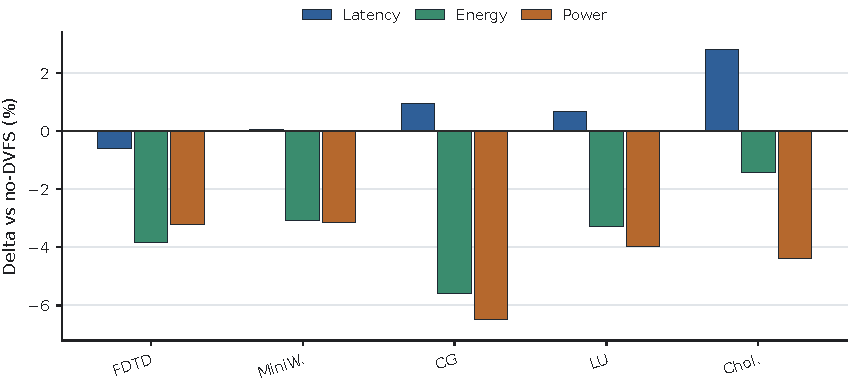
\includegraphics[width=0.94\linewidth]{figures/dvfs_deltas.pdf}
\caption{Per-benchmark DVFS latency, energy, and power deltas relative to no-DVFS execution. The figure reports power together with energy and latency because lower power alone is not sufficient if runtime increases too much.}
\label{fig:results-dvfs-deltas}
\end{figure}%
}

\newcommand{\figDvfsTradeoff}{%
\begin{figure}[!htbp]
\centering
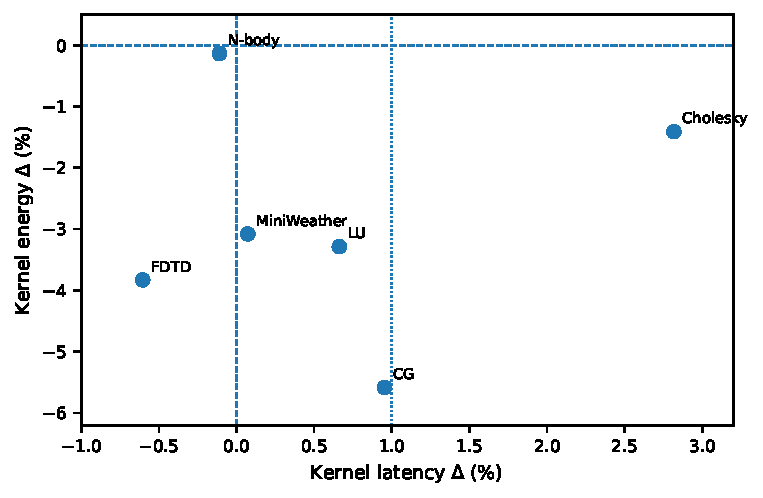
\includegraphics[width=0.78\linewidth]{figures/dvfs_tradeoff.pdf}
\caption{Energy--latency trade-off of WinDVFS. The dotted vertical line marks a 1\% latency-overhead reference. Points below the horizontal axis reduce energy; points to the left of the vertical axis also reduce latency.}
\label{fig:results-dvfs-tradeoff}
\end{figure}%
}

\newcommand{\figDvfsEdpRatios}{%
\begin{figure}[!htbp]
\centering
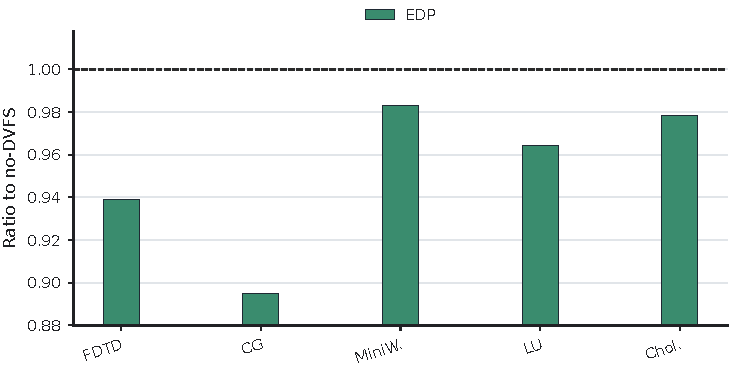
\includegraphics[width=0.94\linewidth]{figures/dvfs_edp_ratios.pdf}
\caption{DVFS EDP ratios relative to no-DVFS execution. Values below the dashed 1.0 line indicate improvement after accounting for runtime.}
\label{fig:results-dvfs-edp-ratios}
\end{figure}%
}

\newcommand{\figMidEnergyScatter}{%
\begin{figure}[!htbp]
\centering
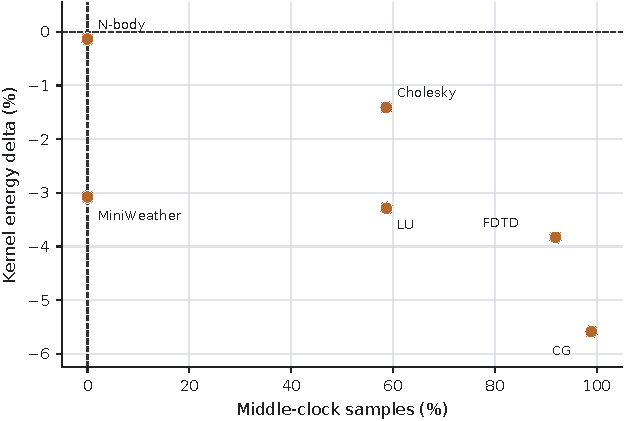
\includegraphics[width=0.78\linewidth]{figures/mid_energy_scatter.pdf}
\caption{Middle-clock sample share and energy reduction. MiniWeather is an exception to a simple residency-based explanation because its measured energy decreases despite zero middle-clock samples.}
\label{fig:results-mid-energy}
\end{figure}%
}

\newcommand{\figDvfsCommitShare}{%
\begin{figure}[!htbp]
\centering
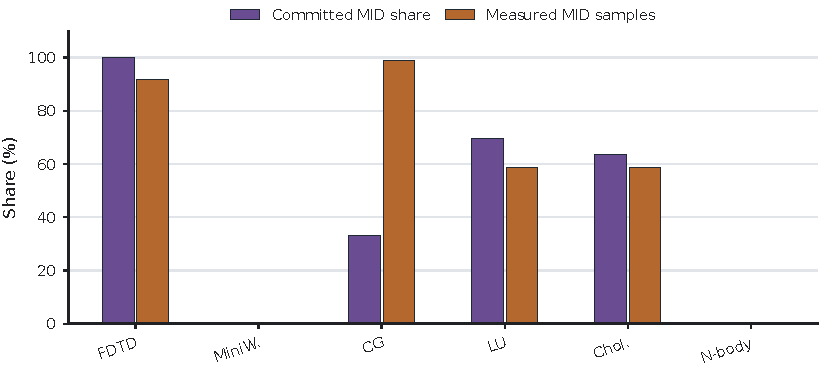
\includegraphics[width=0.94\linewidth]{figures/dvfs_commit_share.pdf}
\caption{Controller-reported committed MID share compared with measured middle-clock sample share. The two quantities are related but not identical because clock samples are collected at NVML sampling timestamps, whereas committed share is reported by the controller.}
\label{fig:results-dvfs-commit-share}
\end{figure}%
}

\newcommand{\figDvfsGuardrailEvents}{%
\begin{figure}[!htbp]
\centering
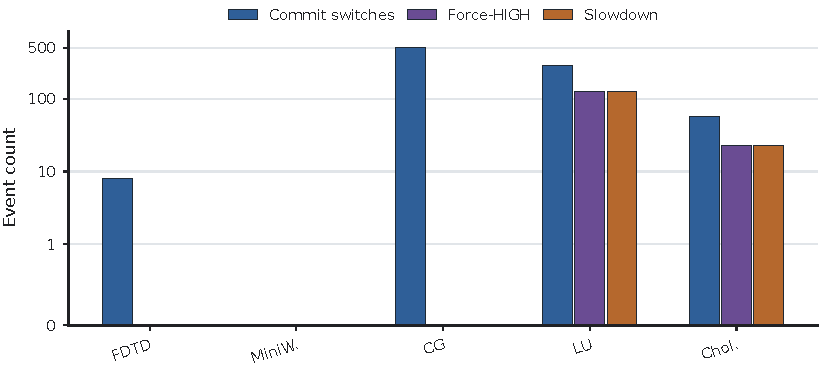
\includegraphics[width=0.94\linewidth]{figures/dvfs_guardrail_events.pdf}
\caption{DVFS commit-switch and guardrail-event counts for the final DVFS measurements. The y-axis uses a symmetric log scale so that zero and small-count workloads can be shown together with CG and LU decomposition.}
\label{fig:results-dvfs-guardrail-events}
\end{figure}%
}

\newcommand{\figOverheadSnapshot}{%
\begin{figure}[!htbp]
\centering
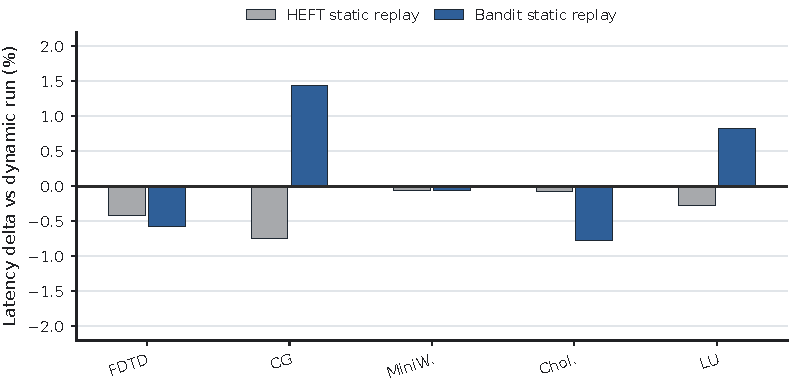
\includegraphics[width=0.86\linewidth]{figures/overhead_snapshot.pdf}
\caption{Diagnostic overhead snapshot for compact placement logging and the WinDVFS diagnostic row. These rows are diagnostic stress checks and are not used to compute the primary placement or DVFS results.}
\label{fig:results-overhead-snapshot}
\end{figure}%
}
